\documentclass[letterpaper,12pt]{article}

\usepackage{graphicx}
\DeclareGraphicsExtensions{.pdf,.png,.gif,.jpg}
\usepackage[usenames,dvipsnames,svgnames,table]{xcolor}
\definecolor{light-gray}{gray}{0.5}
\usepackage{amsmath}
\usepackage{amsthm}
\usepackage[hyperfootnotes=false]{hyperref}
\hypersetup{colorlinks=true,linkcolor=blue,anchorcolor=blue,citecolor=blue,filecolor=blue,urlcolor=blue,bookmarksnumbered=true,pdfview=FitB} %
\usepackage{doi}
\usepackage{tikz}
\usepackage{bm}
\usepackage{tabu}
\usepackage{subfig}
\usepackage{listings}
\usepackage[noabbrev,capitalize]{cleveref}
\newcommand{\mc}[1]{\multicolumn{1}{c}{#1}}
\usepackage{siunitx}
\sisetup{
  %use option "per-mode = reciprocal-positive-first" on a command to make it use e.g. m s^{-1}
  %use option "per-mode = symbol" on a command to make it use e.g. m/s
  per-mode = reciprocal-positive-first,
  binary-units = true,
  %range-phrase = {\text{--}},  % or { to }
  range-phrase = { to },  % or { to }
  %range-units = single,  % or repeat or brackets
  range-units = repeat,  % or repeat or brackets
  list-units = single,  % or repeat or brackets
  multi-part-units = single,  % or repeat or brackets
  separate-uncertainty = true, % use \pm instead of brackets
  mode = text,
  %detect-mode = true,
  %detect-shape = true,
  detect-family = true,
  detect-weight = true
}%
% Remember to always put {} after these commands to fix spacing issues!
\newcommand{\GeV}{\giga\electronvolt}
\newcommand{\GeVc}{\GeV{}\per c}
\newcommand{\GeVcc}{\GeV{}\per\square c}
\newcommand{\TeV}{\tera\electronvolt}
\newcommand{\TeVc}{\TeV{}\per c}
\newcommand{\TeVcc}{\TeV{}\per\square c}
\newcommand{\MeV}{\mega\electronvolt}
\newcommand{\MeVc}{\MeV{}\per c}
\newcommand{\MeVcc}{\MeV{}\per\square c}
\newcommand{\keV}{\kilo\electronvolt}
\newcommand{\keVc}{\keV{}\per c}
\newcommand{\keVcc}{\keV{}\per\square c}
\newcommand{\eV}{\electronvolt}
\newcommand{\eVc}{\eV{}\per c}
\newcommand{\eVcc}{\eV{}\per\square c}

%%% Stuff to print git commit in footer
\usepackage[mark]{gitinfo2}

\newcommand{\pip}{\ensuremath{\pi^{+}}}
\newcommand{\pim}{\ensuremath{\pi^{-}}}
\newcommand{\pipm}{\ensuremath{\pi^{\pm}}}
\newcommand{\pi0}{\ensuremath{\pi^{0}}}
\newcommand{\ep}{\ensuremath{\text{e}^{+}}}
\newcommand{\em}{\ensuremath{\text{e}^{-}}}
\newcommand{\epm}{\ensuremath{\text{e}^{\pm}}}
\newcommand{\gam}{\ensuremath{\gamma}}

\title{Pion Absorption $+$ Charge Exchange Cross-section with LArIAT}
\author{Justin Hugon, William Metcalf, Andrew Olivier,\\Martin Tzanov, Derek Walker}

\begin{document}

\maketitle

\section{Introduction}

When neutrinos interact with argon nuclei, in LArTPCs like MicroBooNE, SBND,
and DUNE, the hadronic recoil consists of charged and neutral pions along with
protons and neutrons. Understanding how these hadrons interact in argon is
important for accurately reconstructing the initial neutrino kinematics.  One
of the main missions of LArIAT is to measure the cross-sections of charged
pions on argon. This note focuses specifically on the pion absorption and
charge exchange pion interactions.

In pion absorption, a charged pion interacts with a nucleus to produce non-pion
hadrons. Protons and neutrons are the most common products of pion absorption,
but deuterons and kaons can also be
produced~\cite{Kotlinski:1998vh,Rowntree:1999dp,Kotlinski:2000hp,Androic:2001tq}.
Neutrons are difficult to detect in a LArTPC because, as neutral particles,
they only produce ionization electrons when they interact with nuclei. Thus,
observations of pion absorption in argon rely on identification of protons,
deuterons, and very rarely kaons.

In pion charge exchange, a charged pion interacts with a nucleus so that the
pion's charge is added to the nucleus and a neutral pion is produced. Neutral
pions decay to a pair of photons, and the short neutral pion lifetime means
that they decay near the nucleus where they were produced. Thus, charge
exchange interactions are similar to pion absorption interactions, but with the
addition of two electromagnetic showers.

\section{Data \& Monte Carlo Samples}

Data for this study comes from LArIAT Run II which took place in 2016. For the
main analysis, only the positive magnet polarity runs are used. Some
cross-checks use the negative polarity runs. The data considered are from the
SAM dataset definitions \texttt{Lovely1\_Pos\_RunII\_elenag\_v04} and
\texttt{Lovely1\_Neg\_RunII\_elenag\_v04} which contain 57219 and 72532 files,
respectively. ``Lovely1'' is the nickname for good subruns where the TPC, WCs,
and ToF is working properly. \cref{tab:samDatasetProps} shows the requirements
in the dataset definitions.

\begin{table}[!hbtp]
  \begin{center}
    \caption{SAM file selection for datasets.}
    \label{tab:samDatasetProps}
    \small
    \begin{tabu}{|p{2.5in}|p{2.4in}|} \hline
      SAM Cut & Explaination \\ \hline \hline
      create\_date $<$ `2017-06-02' & Don't include later processing \\ \hline
      data\_tier digits & Unpacked files \\ \hline
      data\_tier digits & Unpacked files \\ \hline
      lariat\_mid\_f\_mc7anb $<$ 0 or $>$ 0 & Positive or negative magnet polarity \\ \hline
      run\_number $>$= 8000 and run\_number $<$= 10226 & The Run II set of runs \\ \hline
      TPC\_voltages\_nominal & Self-explanatory \\ \hline
      defname: TPC\_MaxGainAndFilter & TPC preamp/shapers set to maximum gain and shaping time (3 \& 3)\\ \hline
      defname: TPC\_nominal\_read\_out\_and\_timing & Normal TPC readout mode \\ \hline
      defname: BothTOF\_OnAndReadOut & Self-explanatory \\ \hline
      defname: AllMWPC\_OnAndReadOut & Self-explanatory \\ \hline
    \end{tabu}
  \end{center}
\end{table}

Additional dataset definitions are for specific secondary beam momenta and
tertiary magnet currents. These are subsets of
\texttt{Lovely1\_Pos\_RunII\_elenag\_v04}. For the nominal momentum and
current, these datasets require the \texttt{secondary.momentum} and
\texttt{tertiary.magnet\_current} to be within one unit of the nominal value in
GeV and A, respectively. \cref{tab:samSpecificDatasets} shows the dataset
definition names. There are no files for 64 GeV secondary beam with magnet
currents between 0 and 59 A. There are 544 files with secondary beam energy
less than 63~GeV and only 189 files for secondary beam energy less than 59 GeV.
There are no files with secondary beam energy greater than 65~GeV.
\cref{fig:datasetConditions} shows the number of files per magnet current,
compared between data in the Run Summary database and SAM database.

% 64 GeV with current < 39: 2787 files
% 64 GeV with current < 19: 2786 files
% 64 GeV with current > 5 <= 11: 0 files
% 64 GeV with current > 0 <= 5: 0 files
% 64 GeV with current = 0: 2786 files
% 64 GeV with current >= 39 & < 59: 0 files
% 64 GeV with current > 61 & < 99: 2 files
% 64 GeV with current > 101: 2 files
% 64 GeV with current >= 39 <= 41: 0 files
% 64 GeV with current >= 19 <= 21: 0 files

\begin{table}[!hbtp]
  \begin{center}
    \caption{SAM dataset definitions for specific secondary beam momenta (in GeV) 
                and tertiary magnet current (in A) and the number of associated files.}
    \label{tab:samSpecificDatasets}
    \small
    \begin{tabu}{|l|l|} \hline
      SAM Dataset Definition Name & Number of Files \\ \hline \hline
      Lovely1\_Pos\_RunII\_jhugon\_current100\_secondary64\_v1   & 36797 \\ \hline
      Lovely1\_Pos\_RunII\_jhugon\_current60\_secondary64\_v1    & 17078 \\ \hline
%      Lovely1\_Pos\_RunII\_jhugon\_current40\_secondary64\_v1    & 0     \\ \hline
%      Lovely1\_Pos\_RunII\_jhugon\_current20\_secondary64\_v1    & 0     \\ \hline
%      Lovely1\_Pos\_RunII\_jhugon\_currentLT19\_secondary64\_v1  & 2786  \\ \hline
      Lovely1\_Pos\_RunII\_jhugon\_current0\_secondary64\_v1     & 2786  \\ \hline
    \end{tabu}
  \end{center}
\end{table}

\begin{figure}[!hbtp]
  \begin{center}
    \subfloat[]{\label{fig:datasetConditions_hist}
          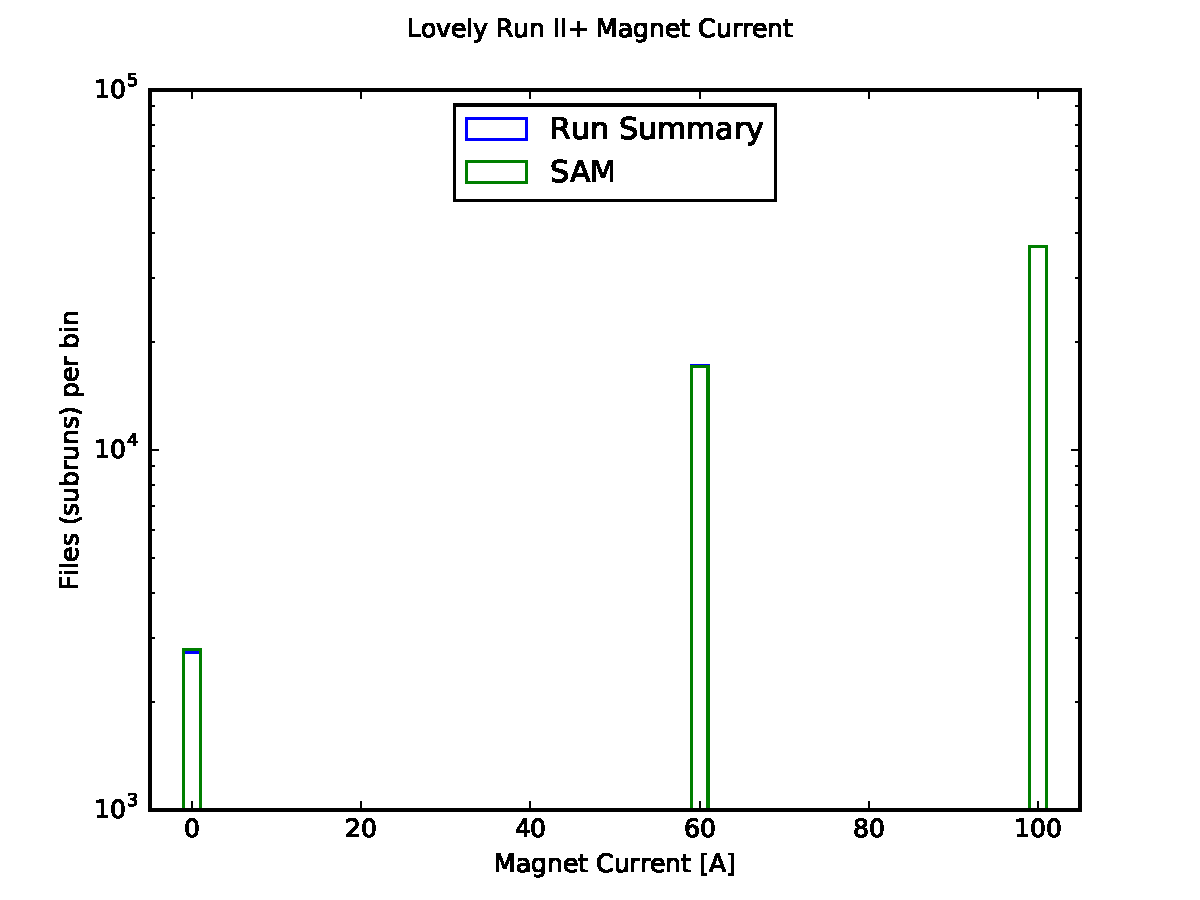
\includegraphics[width=0.48\textwidth]{figures/beamConditions/currentHist.pdf}
    }
    \subfloat[]{\label{fig:datasetConditions_hist2d}
          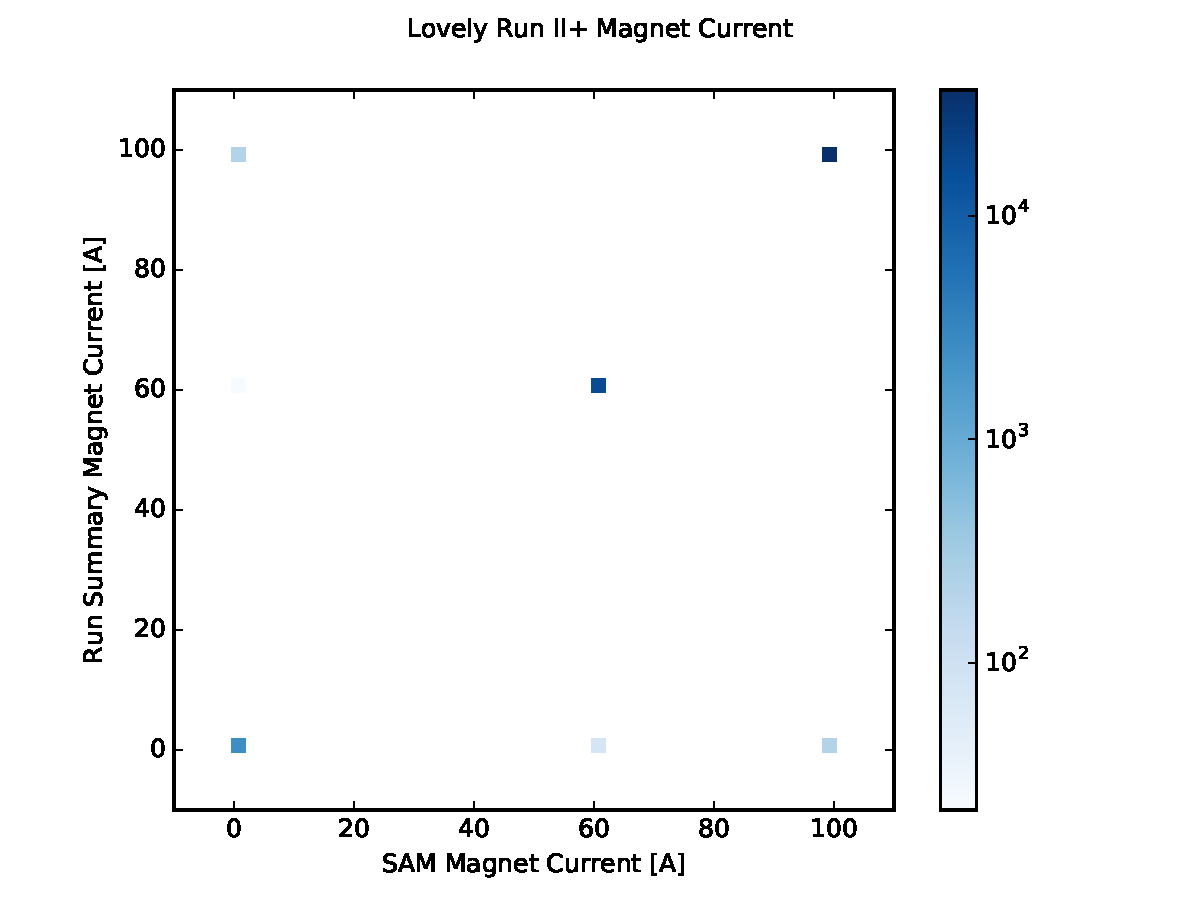
\includegraphics[width=0.48\textwidth]{figures/beamConditions/currentHist2D.pdf}
    }
    \\
    \subfloat[]{\label{fig:datasetConditions_currentVrun}
          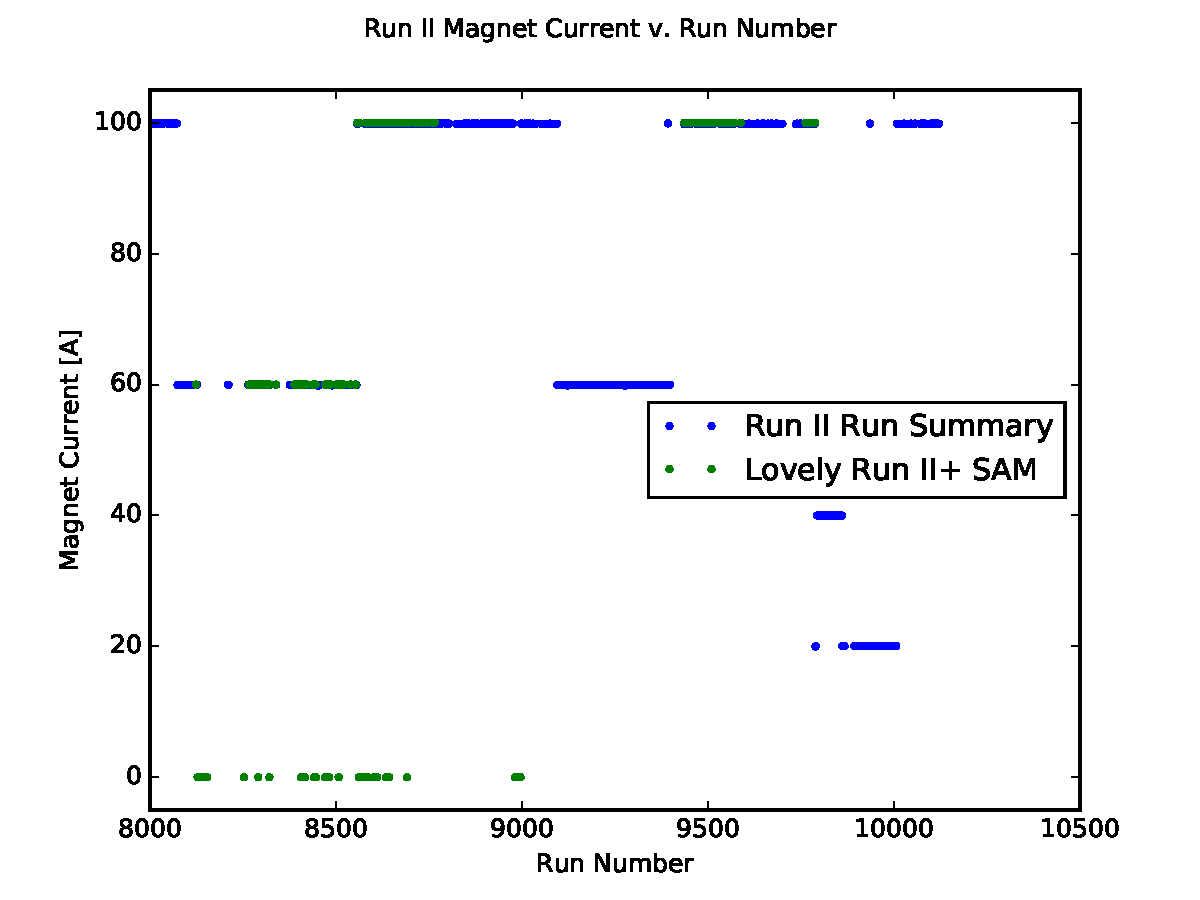
\includegraphics[width=0.48\textwidth]{figures/beamConditions/currentVrun.pdf}
    }
    \caption{%
                Summary plots of the magnet current during Run II. A histogram of 
                magnet current for ``lovely'', positive polarity subruns is 
                shown in \subref{fig:datasetConditions_hist}, the magnet current 
                from the run summary v. SAM is shown in \subref{fig:datasetConditions_hist2d}, 
                and the magnet current v. run number is shown in 
                \subref{fig:datasetConditions_currentVrun}, where the run summary data 
                includes negative polarity and non-lovely runs.
            }
    \label{fig:datasetConditions}
  \end{center}
\end{figure}


The data and MC samples are processed using version v06\_15\_00 of \texttt{larsoft} and
\texttt{lariatsoft}. This software is modified with the git branches listed in
\cref{tab:software}.

\begin{table}[!hbtp]
  \begin{center}
    \caption{Git branch or tag names used for software packages used in this study.}
    \label{tab:software}
    \begin{tabu}{|l|l|} \hline
      \texttt{larsoft} Package & Branch or Tag \\ \hline \hline
      \texttt{lariatsoft} & feature/jhugon\_PionAbsAndChEx \\ \hline
      \texttt{larana} & feature/jhugon\_likelihoodPID\_forlarsoftv06\_15\_00 \\ \hline
      \texttt{larreco} & feature/jhugon\_caloTruth \\ \hline
      \texttt{lardataobj} & feature/jhugon\_caloTruth \\ \hline
      \texttt{larbatch} & c30e15939360 (ups/product\_deps from v06\_15\_00)\\ \hline
    \end{tabu}
  \end{center}
\end{table}

\section{Event Selection}

In this analysis, particles that create hits in the WC, ToF, and TPC are known
as ``primary particles.'' The particles created in interactions of primary
particles are called ``secondary particles.'' These terms also lead to
``primary tracks'' and ``secondary tracks'' that are TPC tracks reconstructed
from primary particles and secondary particles, respectively.

\subsection{Primary \pip{} Selection}

The first part of the selection is meant to identify a pure sample of primary
tracks originating from primary \pip{} particles and called ``primary \pip{}
selection''. The cuts are shown in \cref{tab:pipCuts}. In the data, only events
with PMT flashes in the expected time window of the accelerator cycle for beam
events, \SIrange{1.2}{5.5}{\second}, are selected. Wire chamber tracks must
pass the ``picky track'' cuts, which means that there is exactly one hit on
each X and Y-plane in each of the four WC stations. This is required to ensure
the purest sample of tracks with the best momentum resolution. Since a WC track
is required, this means a single hit is required in each WC plane. The WC
momentum is required to be between \SI{100}{\MeVc{}} and \SI{1100}{\MeVc{}},
and the projected WC track direction must pass through the TPC flange.  The
first reconstructed ToF in the collection is required to between 0 and
\SI{25}{\nano \second}.

To reduce the number of events from \ep{} and beam halo muons as well as
high-occupancy events, some additional cuts are made on TPC tracks. There must
be at least one track in the first \SI{2}{\cm} of the TPC in $z$, while there
must be less than 4 tracks in the first \SI{14}{\cm}. Also, to reduce the \ep{}
contamination, less than 3 tracks with lengths less than \SI{5}{\cm} are
required.

Finally, the WC track must be matched to exactly one TPC track. The cuts are
summarized in \cref{tab:WCTPCMatching}. The matching begins by only looking at
TPC tracks that start in the first \SI{2}{\cm} of the TPC in $z$, and go
through the TPC flange (like the WC tracks). Then all of those TPC tracks and
the WC track are projected to the front face of the TPC (the $z=0$ plane) to
find $x$ and $y$-coordinates. For a WC track and TPC track to match, the
difference in the $x$-coordinates, $\Delta x$, must be between \SI{-4}{\cm} and
\SI{6}{\cm}, and the difference in the $y$-coordinates, $\Delta y$, must be
between \SI{-5}{\cm} and \SI{5}{\cm}. The difference in the 3D angle between
the WC track and TPC track, $\Delta \alpha$, must be less than
\SI{10}{\degree}.

The MC samples are generated using a single particle gun that starts the
primary particle at last WC. There is no WC or ToF information in the MC, and
the PMT information is not used. The assumed WC momentum and direction is set
equal to the initial momentum and direction of the generated primary particle.
Momentum cuts and WC-TPC track matching is then performed in MC just as in
data, using the true initial particle information on position, direction, and
momentum as the WC values. The $\Delta x$ is required to be between
\SI{-5}{\cm} and \SI{5}{\cm}, which differs from the data. This is thought to
be some kind of timing offset in the data that is not present in the MC. The
TPC track cuts are applied just as in data.

\begin{table}[!hbtp]
  \begin{center}
    \small
    \caption{Primary \pip{} selection cuts. See \cref{tab:WCTPCMatching} for WC-TPC track matching.}
    \label{tab:pipCuts}
    \begin{tabu}{|l|l|} \hline
      Variable & Cut \\ \hline \hline
      PMT time stamp & \SIrange{1.2}{5.5}{\second} \\ \hline
      N$_{\text{hits}}$ in each WC plane & 1 \\ \hline
      WC momentum & \SIrange{100}{1100}{\MeVc{}} \\ \hline
      x, y of WC track projected to $z=0$ & $\sqrt{(x-\SI{23.75}{\cm})^2+(y-\SI{0.2}{\cm})^2} < \SI{11.93}{\cm}$ \\ \hline
      First ToF & \SIrange{0}{25}{\nano \second} \\ \hline
      N$_{\text{tracks}}$ in $z<\SI{2}{\cm}$ & $\geq 1$ \\ \hline
      N$_{\text{tracks}}$ in  $z<\SI{14}{\cm}$ & $< 4$ \\ \hline
      N$_{\text{tracks}}$ with length $<\SI{5}{\cm}$ & $< 3$ \\ \hline
      N TPC tracks matched to the WC track & 1 \\ \hline
    \end{tabu}
  \end{center}
\end{table}

\begin{table}[!hbtp]
  \begin{center}
    \small
    \caption{Wire chamber track to TPC track matching cuts.}
    \label{tab:WCTPCMatching}
    \begin{tabu}{|l|l|} \hline
      Variable & Cut \\ \hline \hline
      TPC track start or end $z$ & $<\SI{2}{\cm} \\ \hline
      x, y of TPC track projected to $z=0$ & $\sqrt{(x-\SI{23.75}{\cm})^2+(y-\SI{0.2}{\cm})^2} < \SI{11.93}{\cm}$ \\ \hline
      Tracks projected to $z=0$: $\Delta x$  & Data: \SIrange{-4}{6}{\cm}, MC: \SIrange{-5}{5}{\cm} \\ \hline
      Tracks projected to $z=0$: $\Delta y$  & \SIrange{-5}{5}{\cm} \\ \hline
      3D angle: $\Delta \alpha$  & $<\SI{10}{\degree}$ \\ \hline
    \end{tabu}
  \end{center}
\end{table}

\section{Cross-section Calculation}

\section{Systematic Uncertainties}

\section{Conclusions}

\appendix
\section{Event Displays}

\begin{figure}[!hbtp]
  \begin{center}
    \includegraphics[width=0.7\textwidth]{figures/evd/}
    \caption{%
                Event display of 
            }
    \label{fig:evd_alkdsg}
  \end{center}
\end{figure}

\bibliographystyle{myEPJC}
\bibliography{mybib.bib}

\end{document}
